\documentclass[../report.tex]{subfiles}

\begin{document}
\graphicspath{{img/}{../img/}}

\section*{Target-Projekt}
Indholdet af denne rapport er en projektanalyse af et projekt fra ITU kurset "Second Year Project: Software Development in Large Teams with International Collaboration". I target-projektet skal de studerende fra ITU samarbejde med en gruppe studerende fra Singapore Management University (SMU) om at udvikle et system til at uploade og downloade mediefiler. Systemet kommer til at have to individuelle front-ends, men et delt backend. Derudover skal designet af systemet og samarbejdet med de singaporeanske studerende dokumenteres.

\section*{Problemformulering}
I denne rapport vil der blive svaret p� f�lgende sp�rgsm�l i forhold til target-projektet.
\\ \\	
\textbf{Hvordan kan man planl�gge og udf�re et eksamensprojekt s� som target-projektet?}
\begin{enumerate}
	\item Hvordan kan man planl�gge projektet?
	\item Hvordan kan man estimere hvor lang tid hver aktivitet i target-projektet tager?
	%\item 	Hvordan kan man afveje hvor lang tid man har estimeret projektet tager i forhold til hvor lang tid man har til r�dighed med henblik p� at opn� det bedst mulige resultat?
	\item 	Hvordan kan man v�lge en passende procesmodel i target-projektet?
	%\item 	How can you manage resources and keep the target project on track?
	\item 	Hvilke dele af projektet kunne v�re blevet gjort anderledes for at opn� et bedre resultat?
\end{enumerate}

\section*{Metode}
%To answer the problem statement we will look at the tools used in the target project. Additionally we will apply other tools to the target project and evaluate the different results. Using these tools include doing calculations and creating diagrams.

For at svare p� problemformuleringen vil forskellige metoder til at estimere, planl�gge og udf�re aktiviteter i target-projektet blive analyseret. I target-projektet anvendes Delphi-metoden til at estimere aktiviteter med, en simplificerert version af SCRUM (SCRUM-but) som procesmodel og et Gantt-chart til planl�gning af aktiviteter. For at indsamle data til brug i denne rapport, blev gruppen i target-projektet bedt om at tage tid p� aktiviteterne de udf�rte. Derudover blev gruppen interviewet omkring forskellige faktorer i target-projektet, og der blev givet tilladelse til at gennemg� al dokumentation vedr�rende target-projektet (user stories, requirements, diagrammer, Scrum boards etc.). Disse data vil blive brugt i forbindelse med analysen af estimeringsmetoder. Derudover vil der sidel�bende blive afpr�vet alternative metoder som kan sammenlignes med de metoder der faktisk blev brugt i projektet. Dette vil inkludere et Precendence Network til planl�gning af aktiviteter, Use Case Points og PERT til estimering og vandfaldsmodellen som procesmodel.

%Forskellige estimeringsmetoder: FP, Delphi
%Forskellige processmodeller: Vandfald, SCRUM, spiral
%Forskellige aktivitetsplanl?gningsmetoder: precedence network (critical path), gantt


\section{Tidsplan} \todo Find ud af, hvad der skal ske med tidsplanen: her, appendix eller v�k? \\

Herunder er tidsplanen for dette projekt

\begin{figure}[H]
\hspace*{-2cm}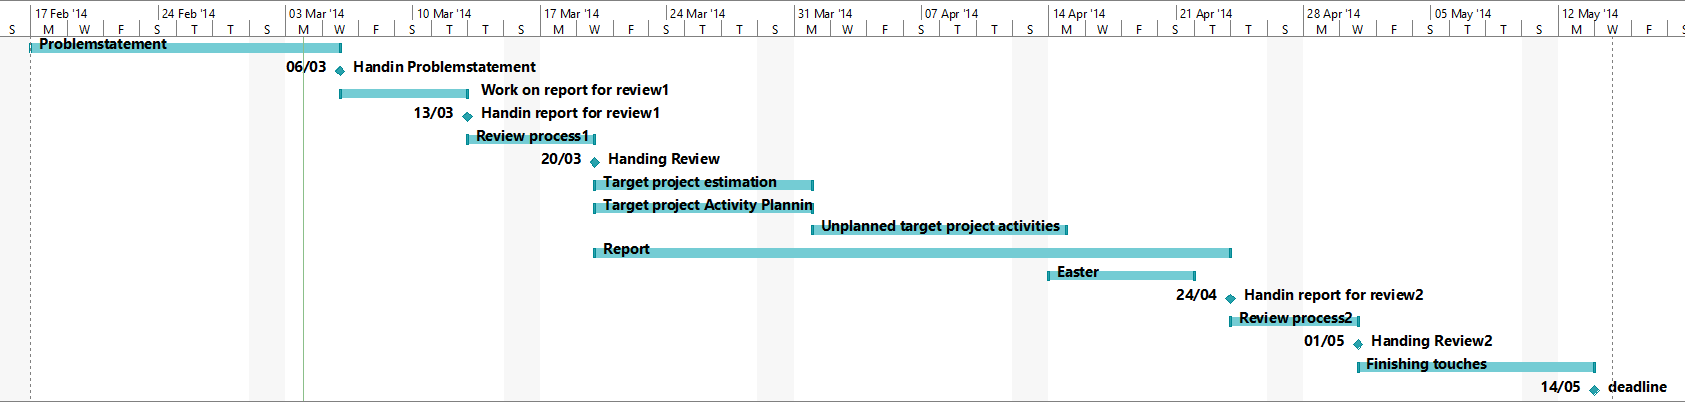
\includegraphics[scale=0.425]{timeschedule.png}
\end{figure}


\end{document}
